\documentclass{article}
\usepackage{graphicx}
\usepackage{wrapfig}
\usepackage{filecontents}
\usepackage{siunitx}
\usepackage[table]{xcolor}
\usepackage{float}
\usepackage{hyperref}

\usepackage{color} % balíček pro obarvování textů
\usepackage{xcolor}  % zapne možnost používání barev, mj. pro \definecolor
\usepackage{pgfplots} % http://www.chiark.greenend.org.uk/doc/texlive-doc/latex/pgfplots/pgfplots.pdf

\ifnum 0\ifxetex 1\fi\ifluatex 1\fi=0 % if pdftex
  \usepackage[T1]{fontenc}
  \usepackage[utf8]{inputenc}
\else % if luatex or xelatex
  \ifxetex
    \usepackage{mathspec}
  \else
    \usepackage{fontspec}
  \fi
  \defaultfontfeatures{Ligatures=TeX,Scale=MatchLowercase}
\fi
\usepackage[total={175mm,230mm}, top=23mm, left=20mm, includefoot]{geometry}
\hypersetup{
    colorlinks,
    linkcolor={blue!50!black},
    citecolor={green!50!black},
    urlcolor={blue!80!black}
}
\definecolor{orange}{RGB}{ 251, 114, 032}
\definecolor{fialova}{RGB}{ 255, 000, 255}

\newcommand \obr[1]
{ obr.~\ref{#1}}

\newcommand \tab[1]
{ tab.~ß\ref{#1}}


\begin{document}
\section{Pracovní bod a jeho pohyb}

Tranzistor je typická nelineární součástka v obvodu popsatelná šesti veličinami, třemi proudy a třemi napětími vyznačenými na \obr{pracovni_bod_tranzistoru} a) (\(I_C I_B I_E U_{CE} U_{BE} U_{BC})\).
Tyto veličiny jsou propojeny nelineárními závislostmi které lze chápat jako šestirozměrný objekt.
Když tímto objektem provede dvourozměrný řez můžeme dostat např. výstupní charakteristiku (závislost \(I_C\) na \(U_{CE}\)
při konstantním proudu \(I_B\)).
\vspace{-1mm}
\begin{figure}[H]
    % \centering
    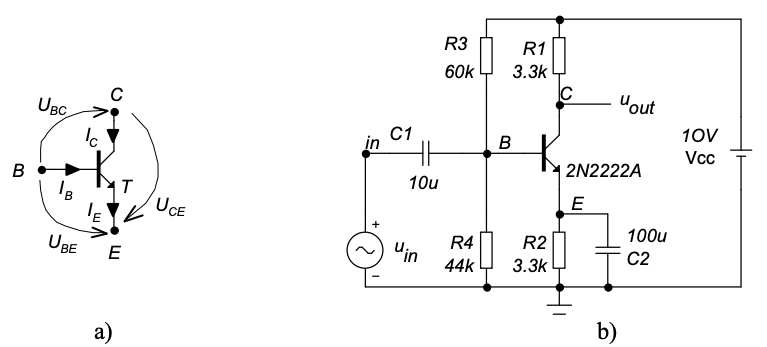
\includegraphics[width=\textwidth]{pracovni_bod_tranzistoru.png}
    \caption{\label{pracovni_bod_tranzistoru}}
\end{figure}


\vspace{1mm}
\begin{wrapfigure}{r}{0.45\textwidth}
  % \centering
  \vspace{-5mm}
  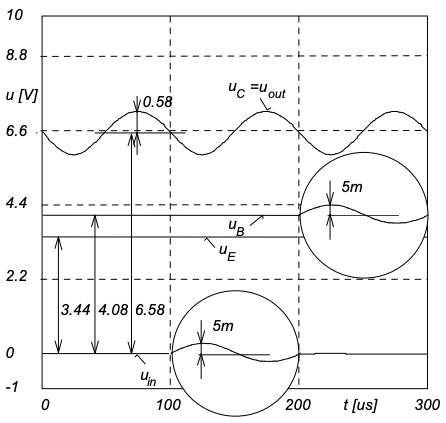
\includegraphics[width=0.5\textwidth]{vstup-baze-vystup.png}
  \caption{\label{vstup_baze_vystup}}
\end{wrapfigure}
Proud kolektorem tranzistoru je určován proudem do báze podle jednoduchého vztahu \(I_C = I_B\cdot\beta\) kde \(\beta \) je proudový zesilovací činitel bipolárního tranzistoru.
Pokud tranzistor zapojíme podle schematu na \obr{pracovni_bod_tranzistoru}~b) při \(U_{in} = 0\) ustálí se jeho veličiny na konkrétním bodě, tento bod označujeme \(Q\) a nazýváme ho stejnosměrný pracovní bod tranzistoru. 
Proud je v tomto zapojení určen odporem \(R_b\) a proudovým zesilovacím činitelem \(\beta\).
Napětí na kolektoru je pak určeno napájecím napětím \(U_{cc}\) a odporem \(R_1\).

Aby mohl tranzistor fungovat správně jako zesilovač, je nutné, aby nastavení pracovního bodu umožňovalo dostatečný rozkmit výstupního signálu oběma směry bez přílišného zkreslení.
Pracovní bod se proto obvykle nastavuje tak aby v ustáleném stavu platilo \(U_{out} = \frac{1}{2}V_{cc}\)

Abychom mohli na tento zesilovač přivést signál s libovolnou stejnosměrnou složkou, přípojíme vstup zesilovače na bázi skrz kapacitu \(C_1\).
Tato kapacita musí být dostatečně velká aby se pro signál o požadované frekvenci dala považovat za zkrat.
Na \obr{vstup_baze_vystup} je zobrazen možný procházející signál.

Šířka pásma zesilovače je rozdíl mezi nejvyšší a nejnižší frekvencí přenášeného signálu.
Při mezní frekvenci dojde k poklesu zesílení o 3dB oproti nejvyššímu zesílení.

\newpage

\section{Počítačové cvičení}
\begin{figure}[H]
  \begin{minipage}[t]{0.5\textwidth}
    \subsection{Bipolární tranzistor}
  \end{minipage}
  \begin{minipage}[t]{0.5\textwidth}
    \vspace{-15mm}
    \begin{figure}[H]
      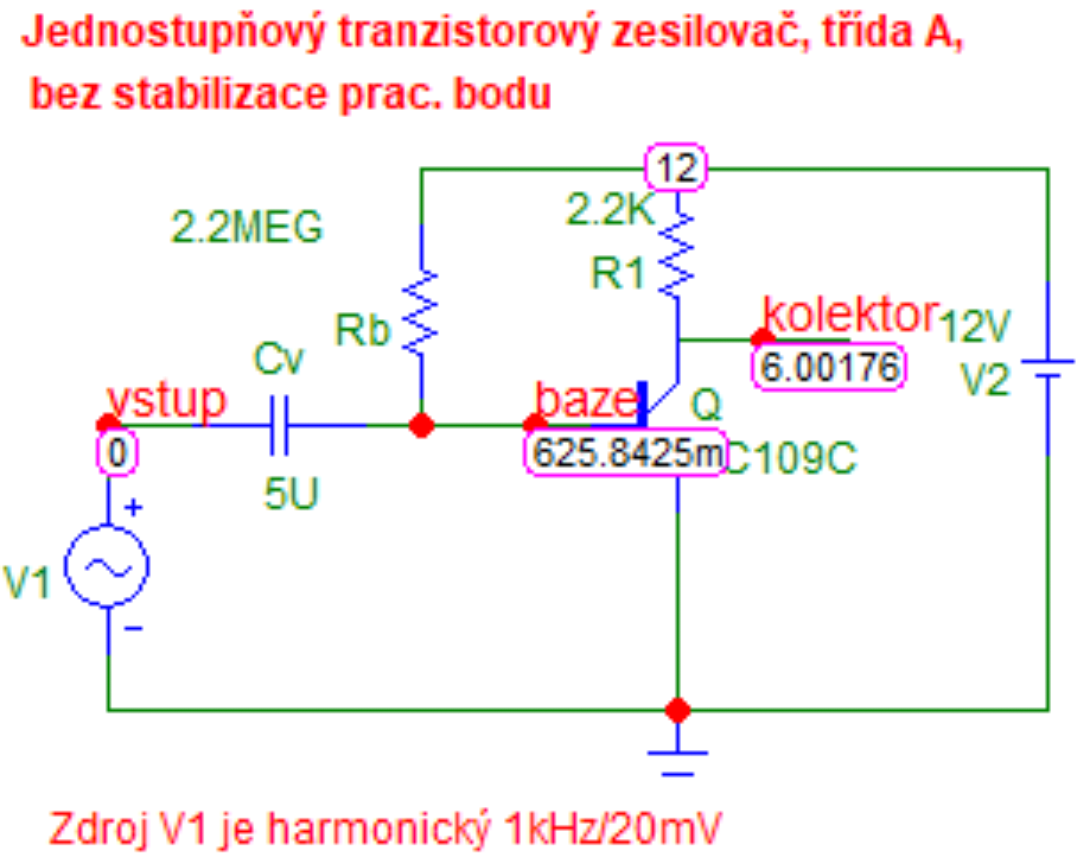
\includegraphics[width=\textwidth]{PC/BJT/prac_bod.png}
      % \addlegendentry{test}
      \caption{\label{prac_bod} Stejnosměrné nastavení pracovního bodu}
    \end{figure}
  \end{minipage}
  
  \begin{minipage}[t]{0.33\textwidth}
    \begin{figure}[H]
      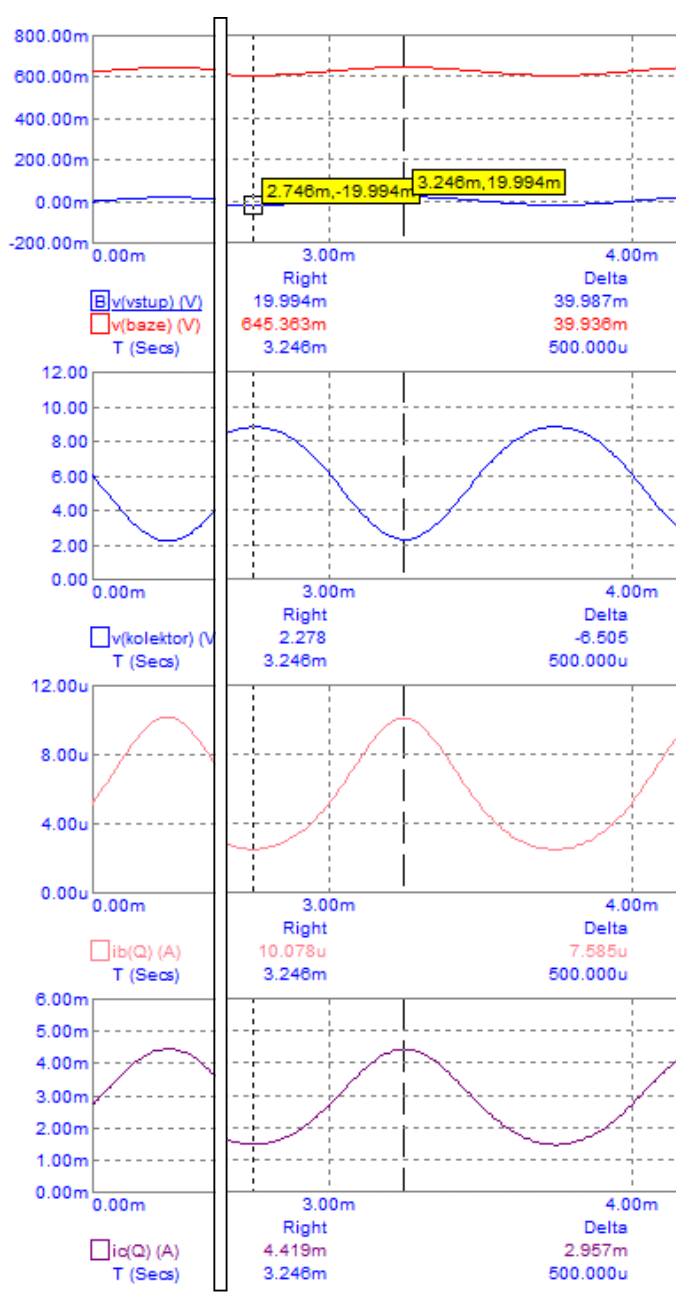
\includegraphics[width=\textwidth]{PC/BJT/sim_1.png}
      % \addlegendentry{test}
      \caption{\label{sim_1} Odezva na základní sinusoví signál}
    \end{figure}
  \end{minipage}
  \hfill
  \begin{minipage}[t]{0.25\textwidth}
    \begin{figure}[H]
      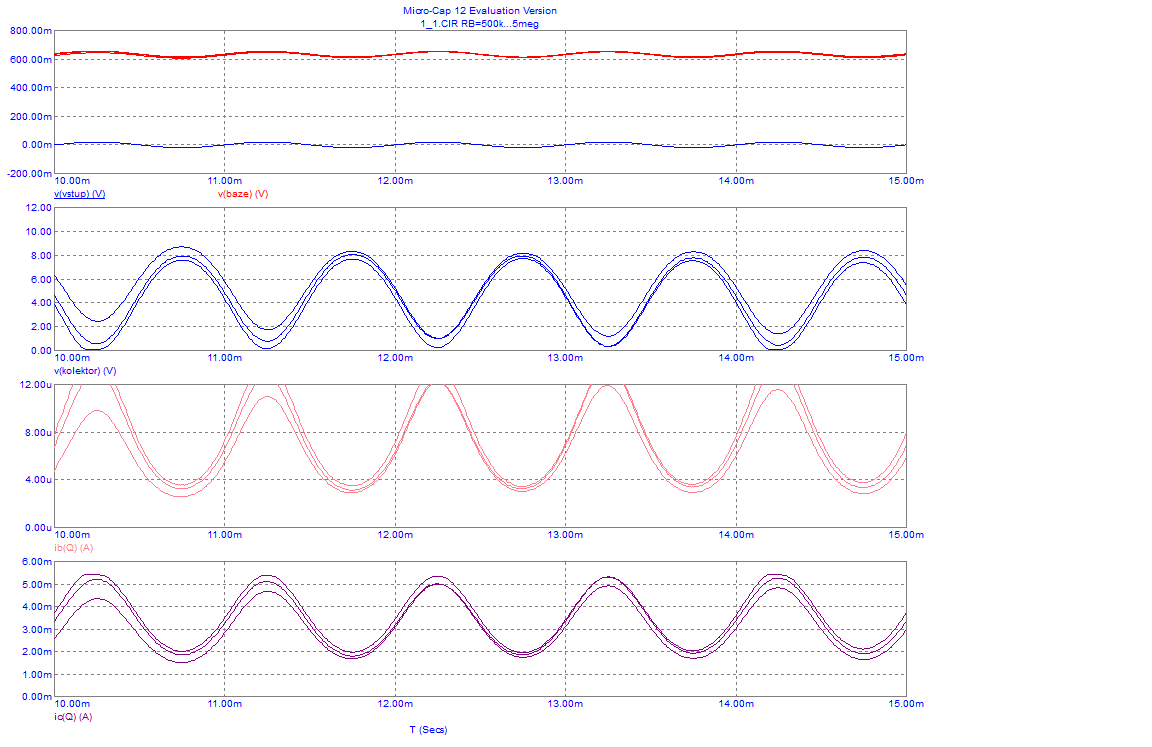
\includegraphics[width=\textwidth]{PC/BJT/Tranzient_analyza_4.png}
      \caption{\label{Tranzient_analyz_4} Sinusový průběh při změně \(R_b\)}
    \end{figure}
  \end{minipage}
  \hfill
  \begin{minipage}[t]{0.3\textwidth}
    \begin{figure}[H]
      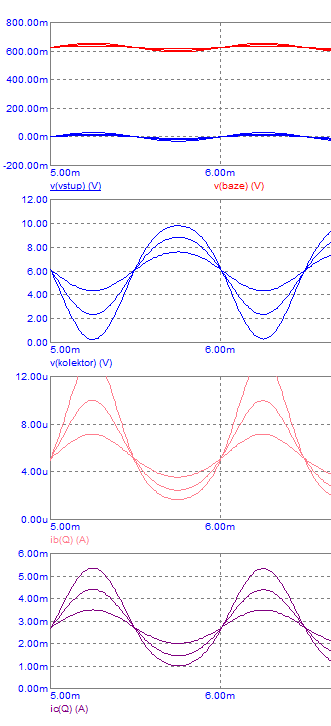
\includegraphics[width=\textwidth]{PC/BJT/Tranzient_analyza_3.png}
      \caption{\label{Tranzient_analyz_5 } Sinusový průběh při změně \(U_{in}\)}
    \end{figure}
  \end{minipage}
\end{figure}

\hfill

\begin{figure}[H]
  \begin{minipage}[t]{\textwidth}
    \begin{figure}[H]
      \includegraphics[width=\textwidth]{PC/BJT/Sirka_pasma.png}
      \caption{\label{sirka_pasma} Šířka pásma při \(C_v = 5\-[\mu F]\)}
    \end{figure}
    \begin{figure}[H]
      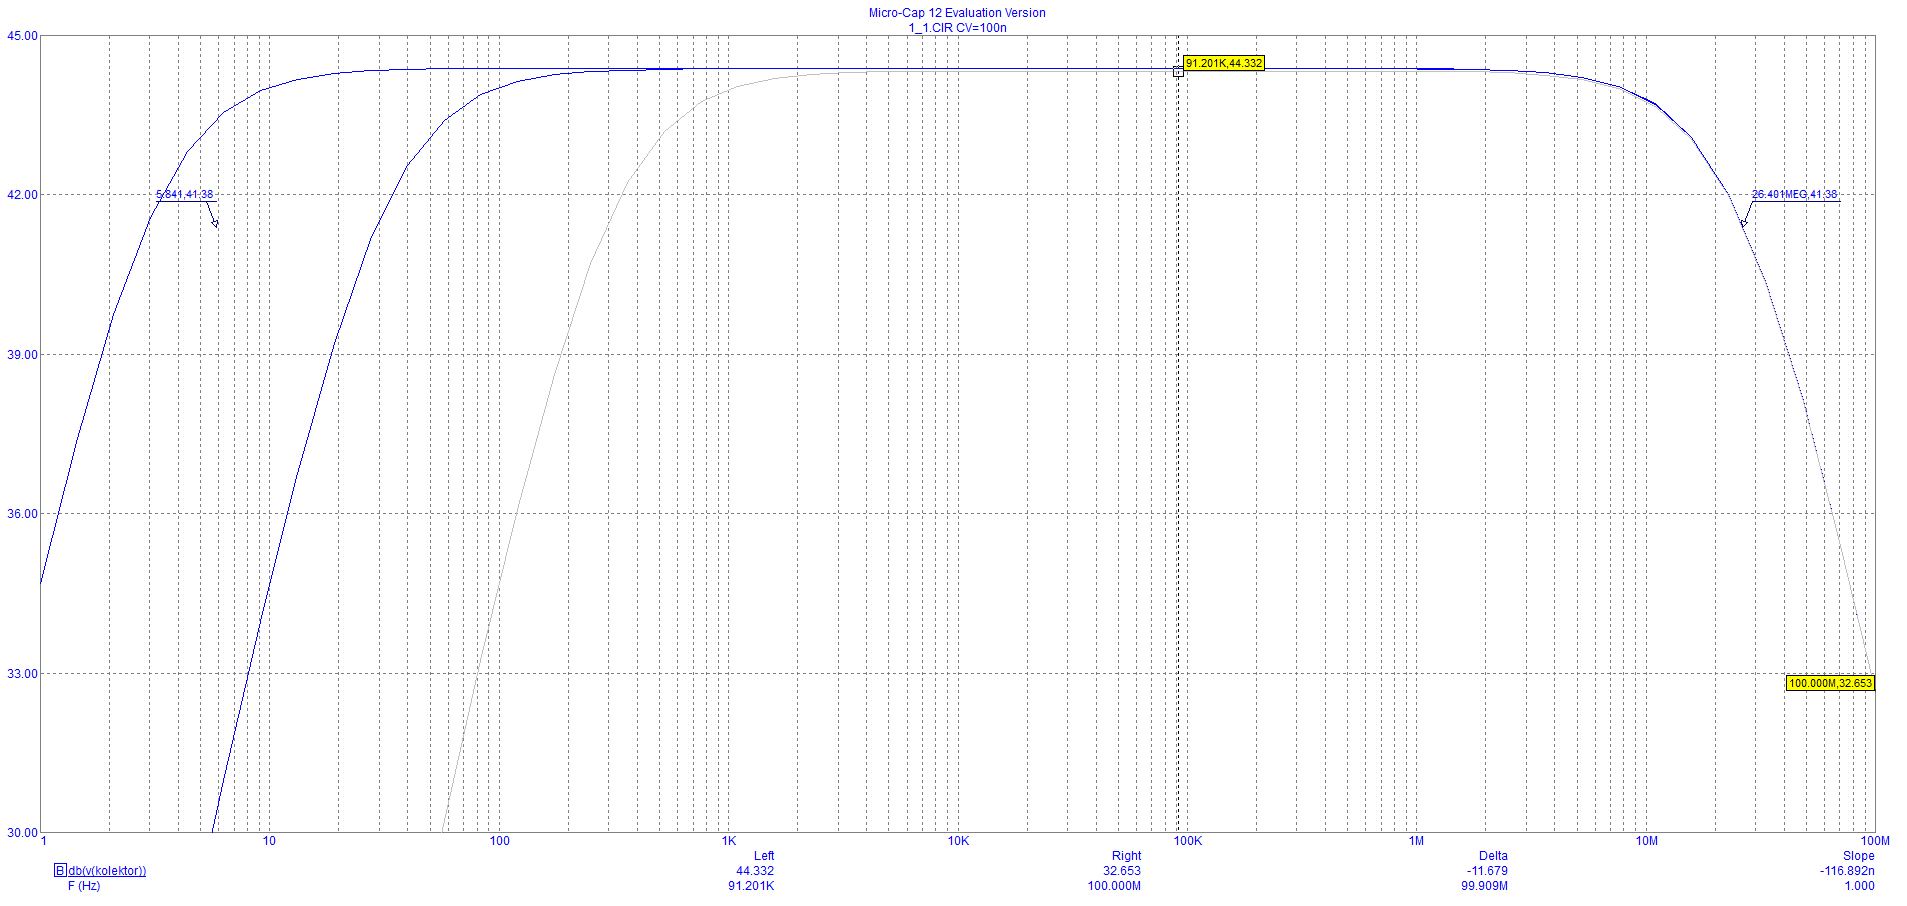
\includegraphics[width=\textwidth]{PC/BJT/Step_sirka_pasma.png}
      \caption{\label{Pohyb_sirky_pasma} Šířka pásma při změně \(C_v = 0.1;1;10\-[\mu F]\)}
    \end{figure}
  \end{minipage}


  \begin{minipage}[t]{\textwidth}
    \vspace{10mm}
    Je vidět že zmenšení kapacitoru znamená omezení šířky pásma v dolní části, nikoliv v horní.
  \end{minipage}
\end{figure}

\newpage

\begin{figure}[H]
  \begin{minipage}[t]{0.4\textwidth}
    \subsection{Unipolární tranzistor}
  \end{minipage}
  \begin{minipage}[t]{0.6\textwidth}
    \begin{figure}[H]
      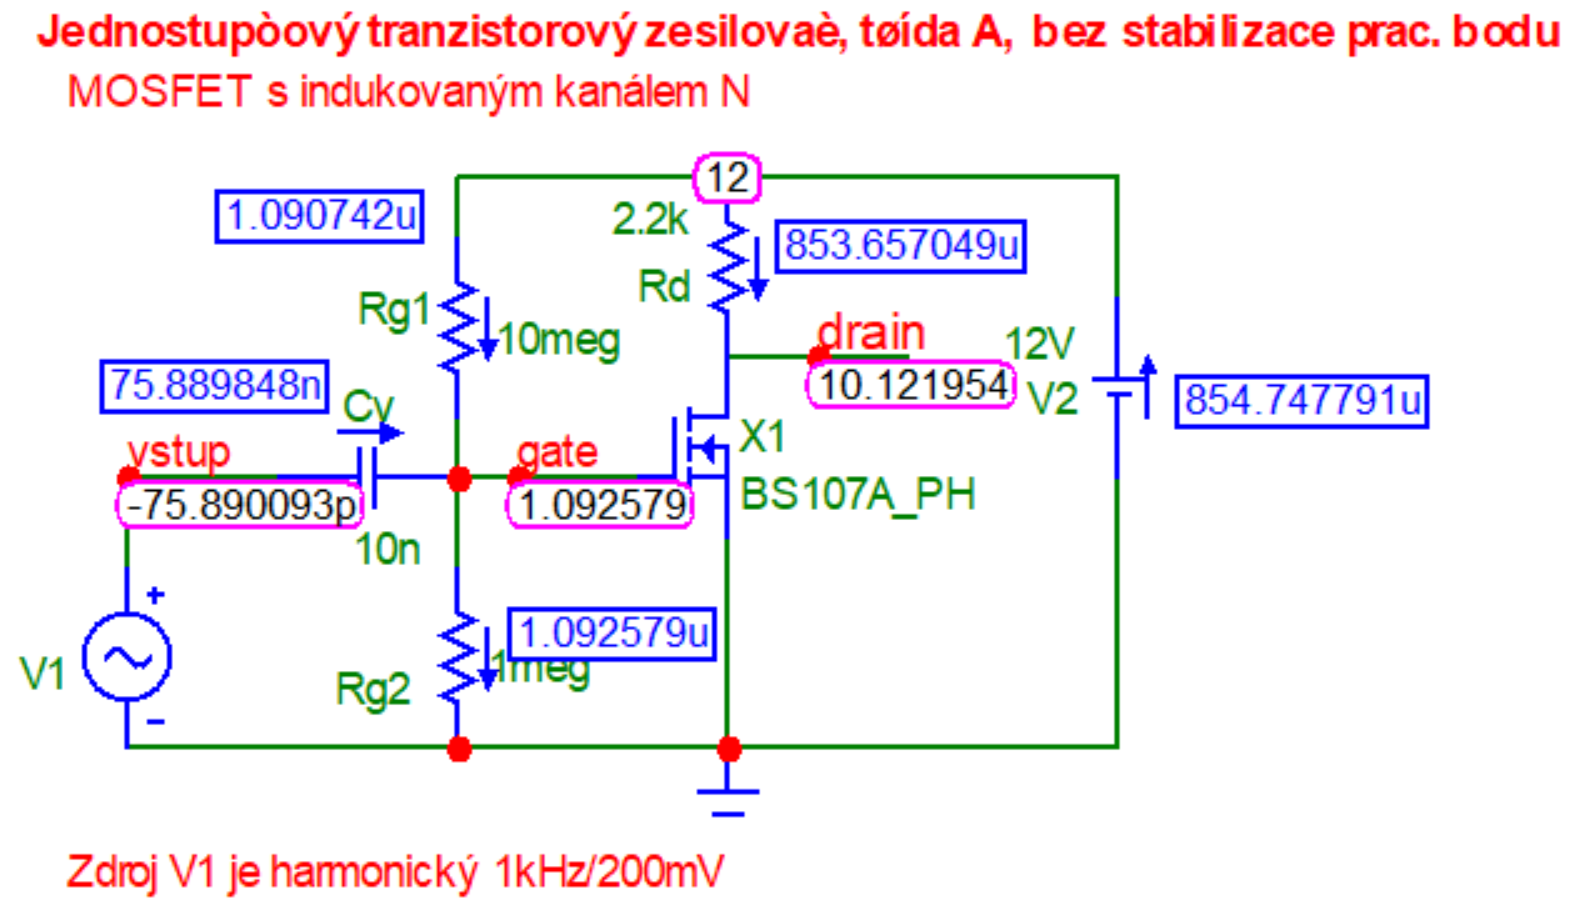
\includegraphics[width=\textwidth]{PC/UNI/napeti_a_proudy.png}
      \caption{\label{UNI_naperi_a_proudy} Stejnosměrné nastavení pracovního bodu}
    \end{figure}
  \end{minipage}
  
  \begin{minipage}[t]{0.30\textwidth}
    \begin{figure}[H]
      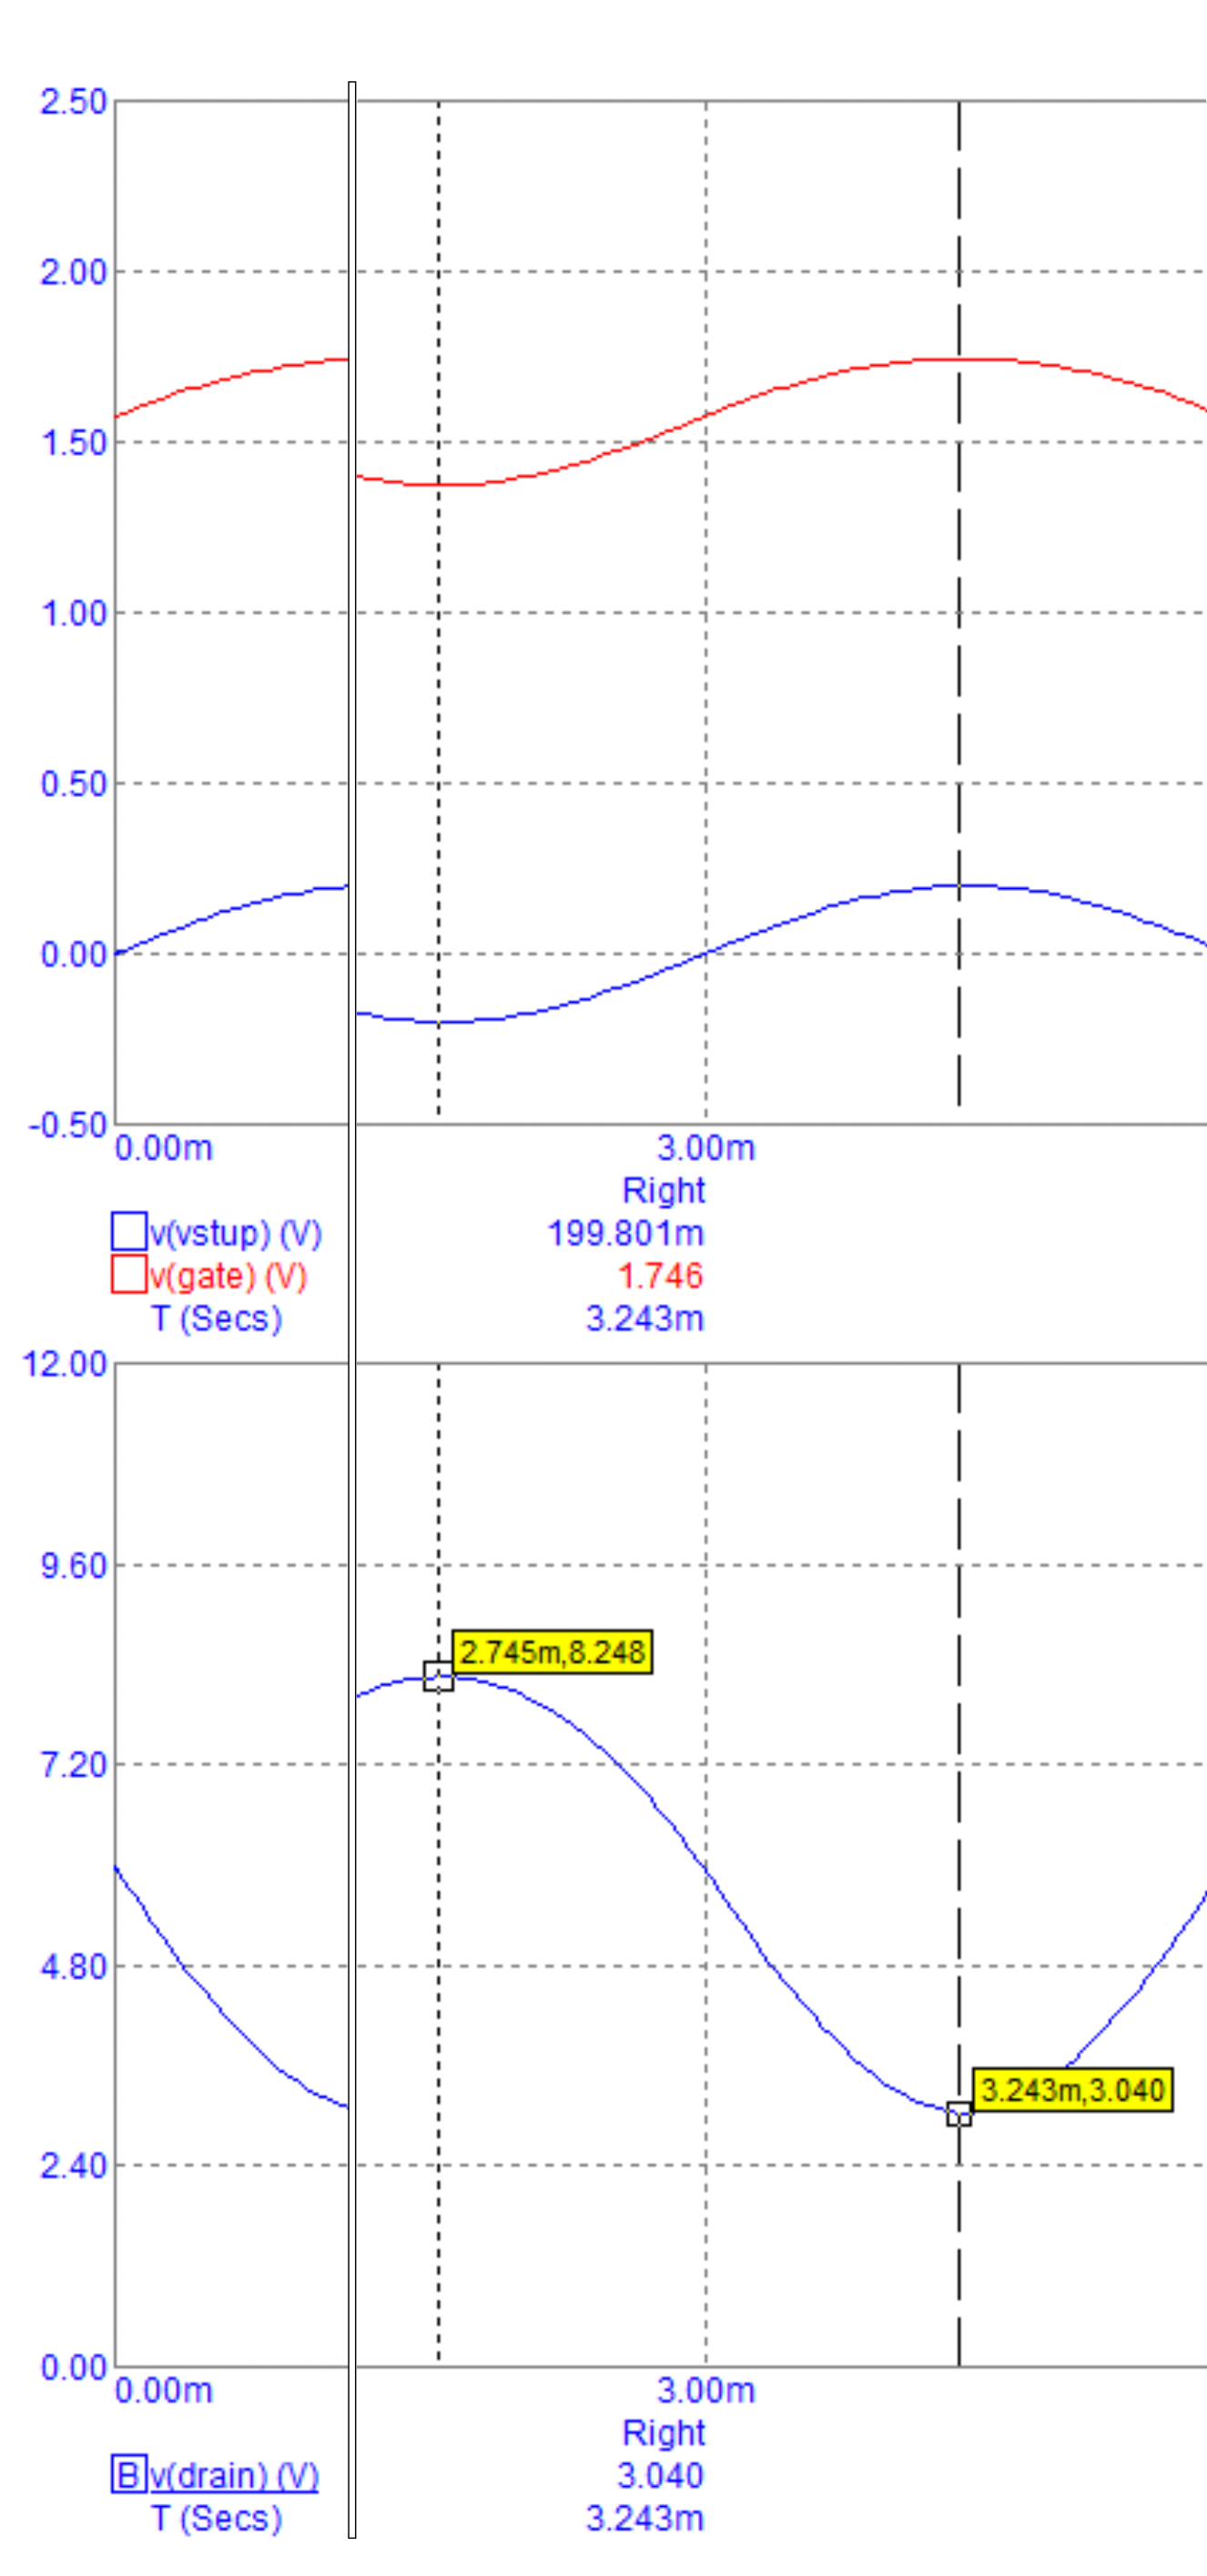
\includegraphics[width=\textwidth]{PC/UNI/UNI_Tranzient_1_3_redukovano.png}
      \caption{\label{UNI_Tranzient_reduk_1} Odezva na základní sinusoví signál}
    \end{figure}
  \end{minipage}
  \hfill
  \begin{minipage}[t]{0.33\textwidth}
    \begin{figure}[H]
      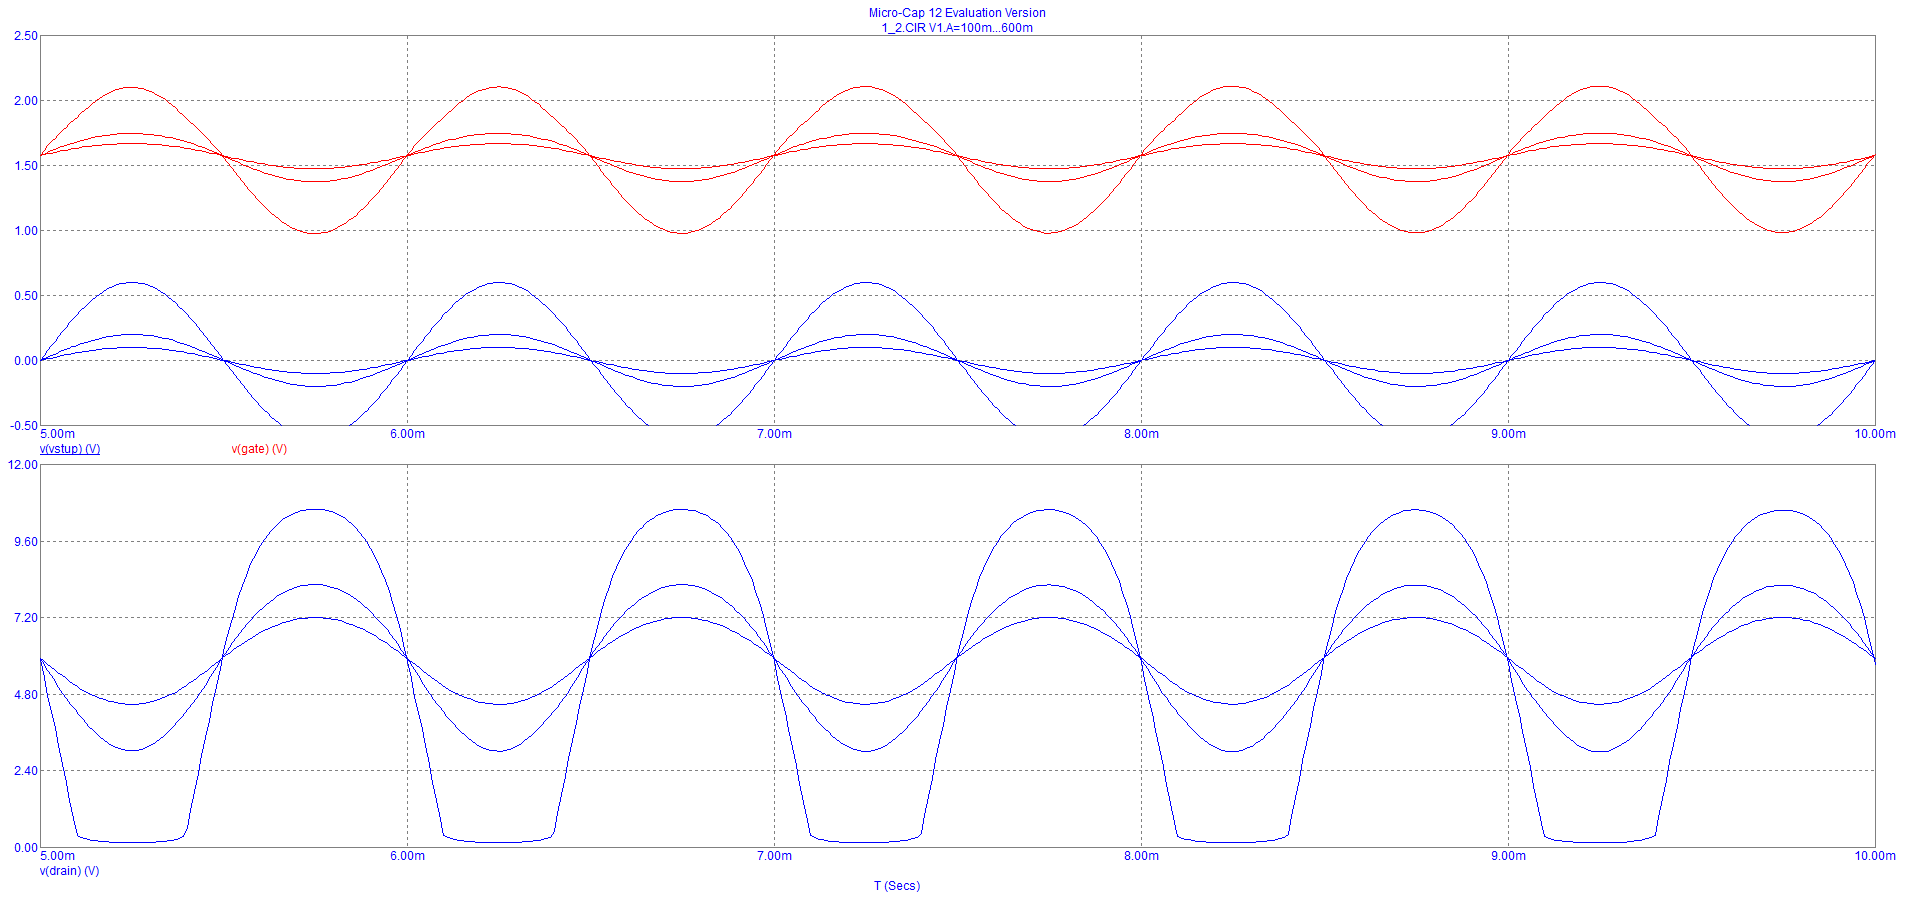
\includegraphics[width=\textwidth]{PC/UNI/UNI_Tranzient_2_1.png}
      \caption{\label{NUI_Tranzient_2} Sinusový průběh při změně \(R_b\)}
    \end{figure}
  \end{minipage}
  \hfill
  \begin{minipage}[t]{0.35\textwidth}
    \begin{figure}[H]
      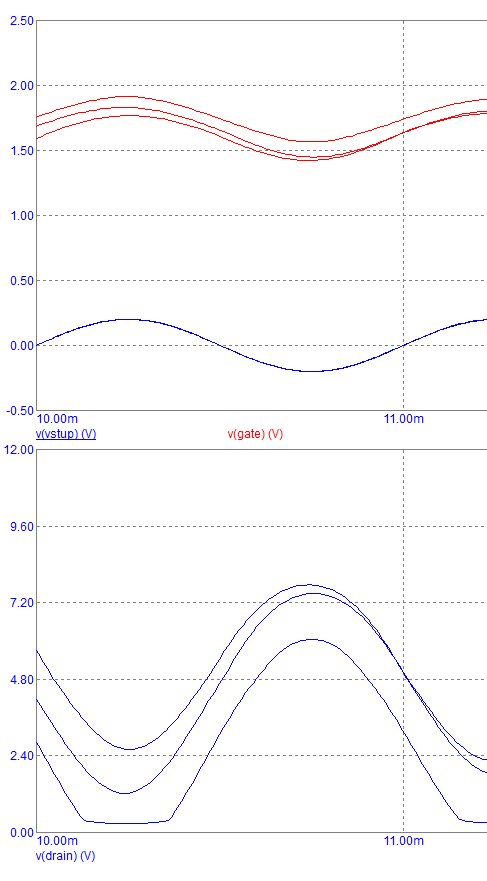
\includegraphics[width=\textwidth]{PC/UNI/posun_prac_podu.png}
      \caption{\label{Posun_prac_bodu} Sinusový průběh při změně \(U_{in}\)}
    \end{figure}
  \end{minipage}
\end{figure}

\begin{figure}[H]
	% \begin{minipage}[t]{0.45\textwidth}
  %   \vspace{-5mm}
  %   \begin{figure}[H]
  %     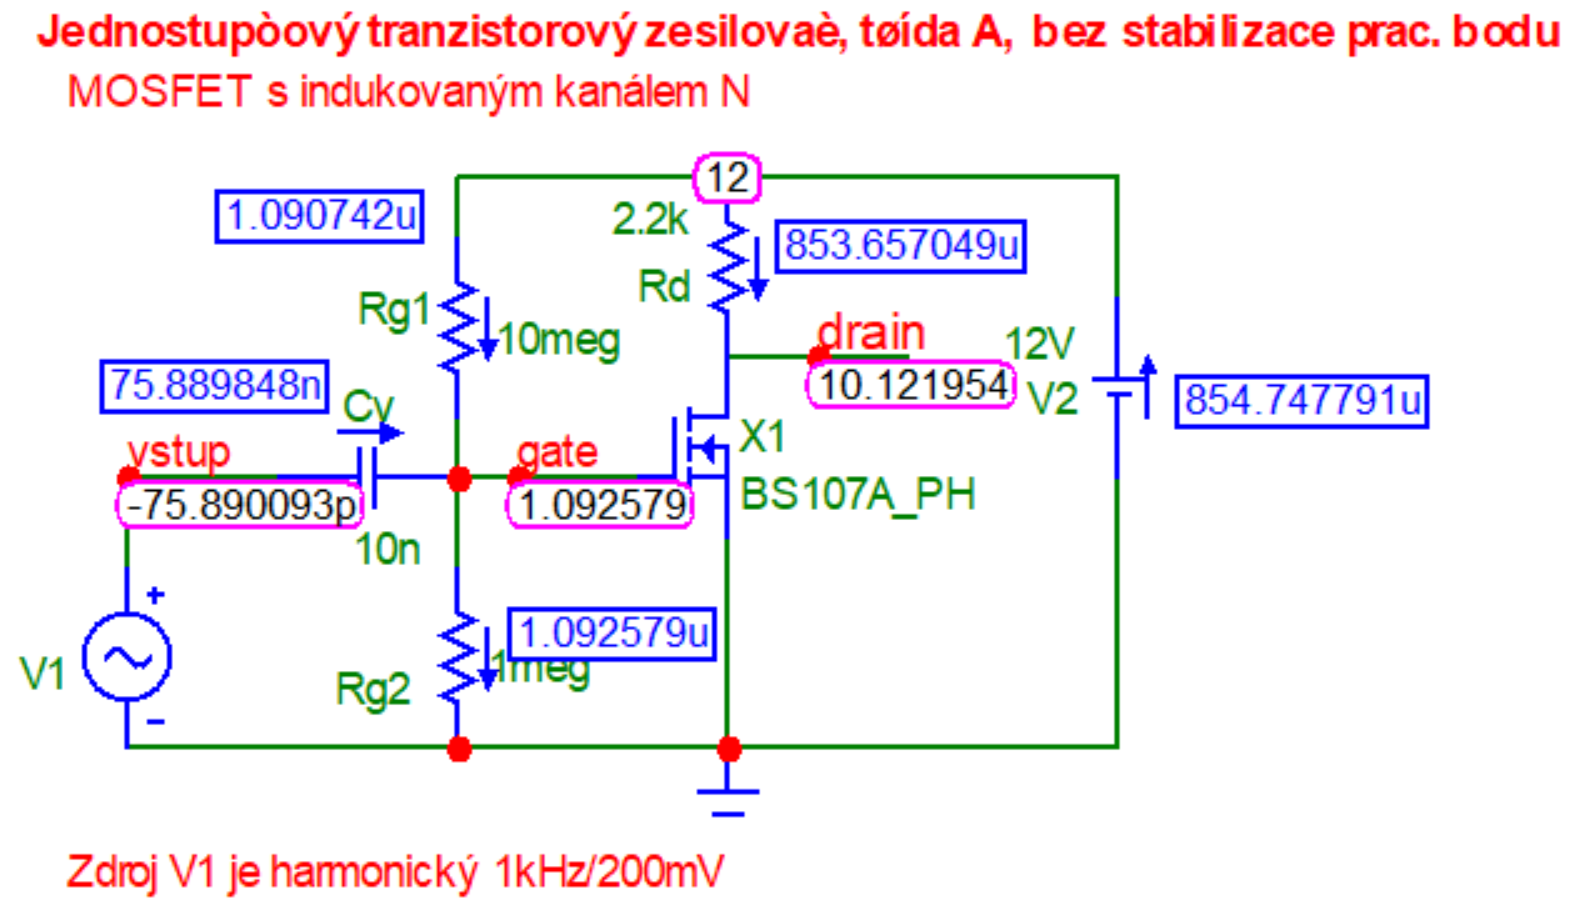
\includegraphics[width=\textwidth]{PC/UNI/napeti_a_proudy.png}
  %     % \addlegendentry{test}
  %     \caption{\label{prac_bod_sim_1} Stejnosměrné nastavení pracovního bodu}
  %   \end{figure}
  % \end{minipage}
  \hfill
  \begin{minipage}[t]{0.45\textwidth}
    \vspace{-10mm}
    \begin{figure}[H]
      % \addlegendentry{test}
      \caption{\label{prac_bod_sim_1} Odezva na základní sinusoví signál}
    \end{figure}
  \end{minipage}
\end{figure}


\begin{figure}[H]
	\begin{minipage}[t]{1\textwidth}
    \begin{figure}[H]
      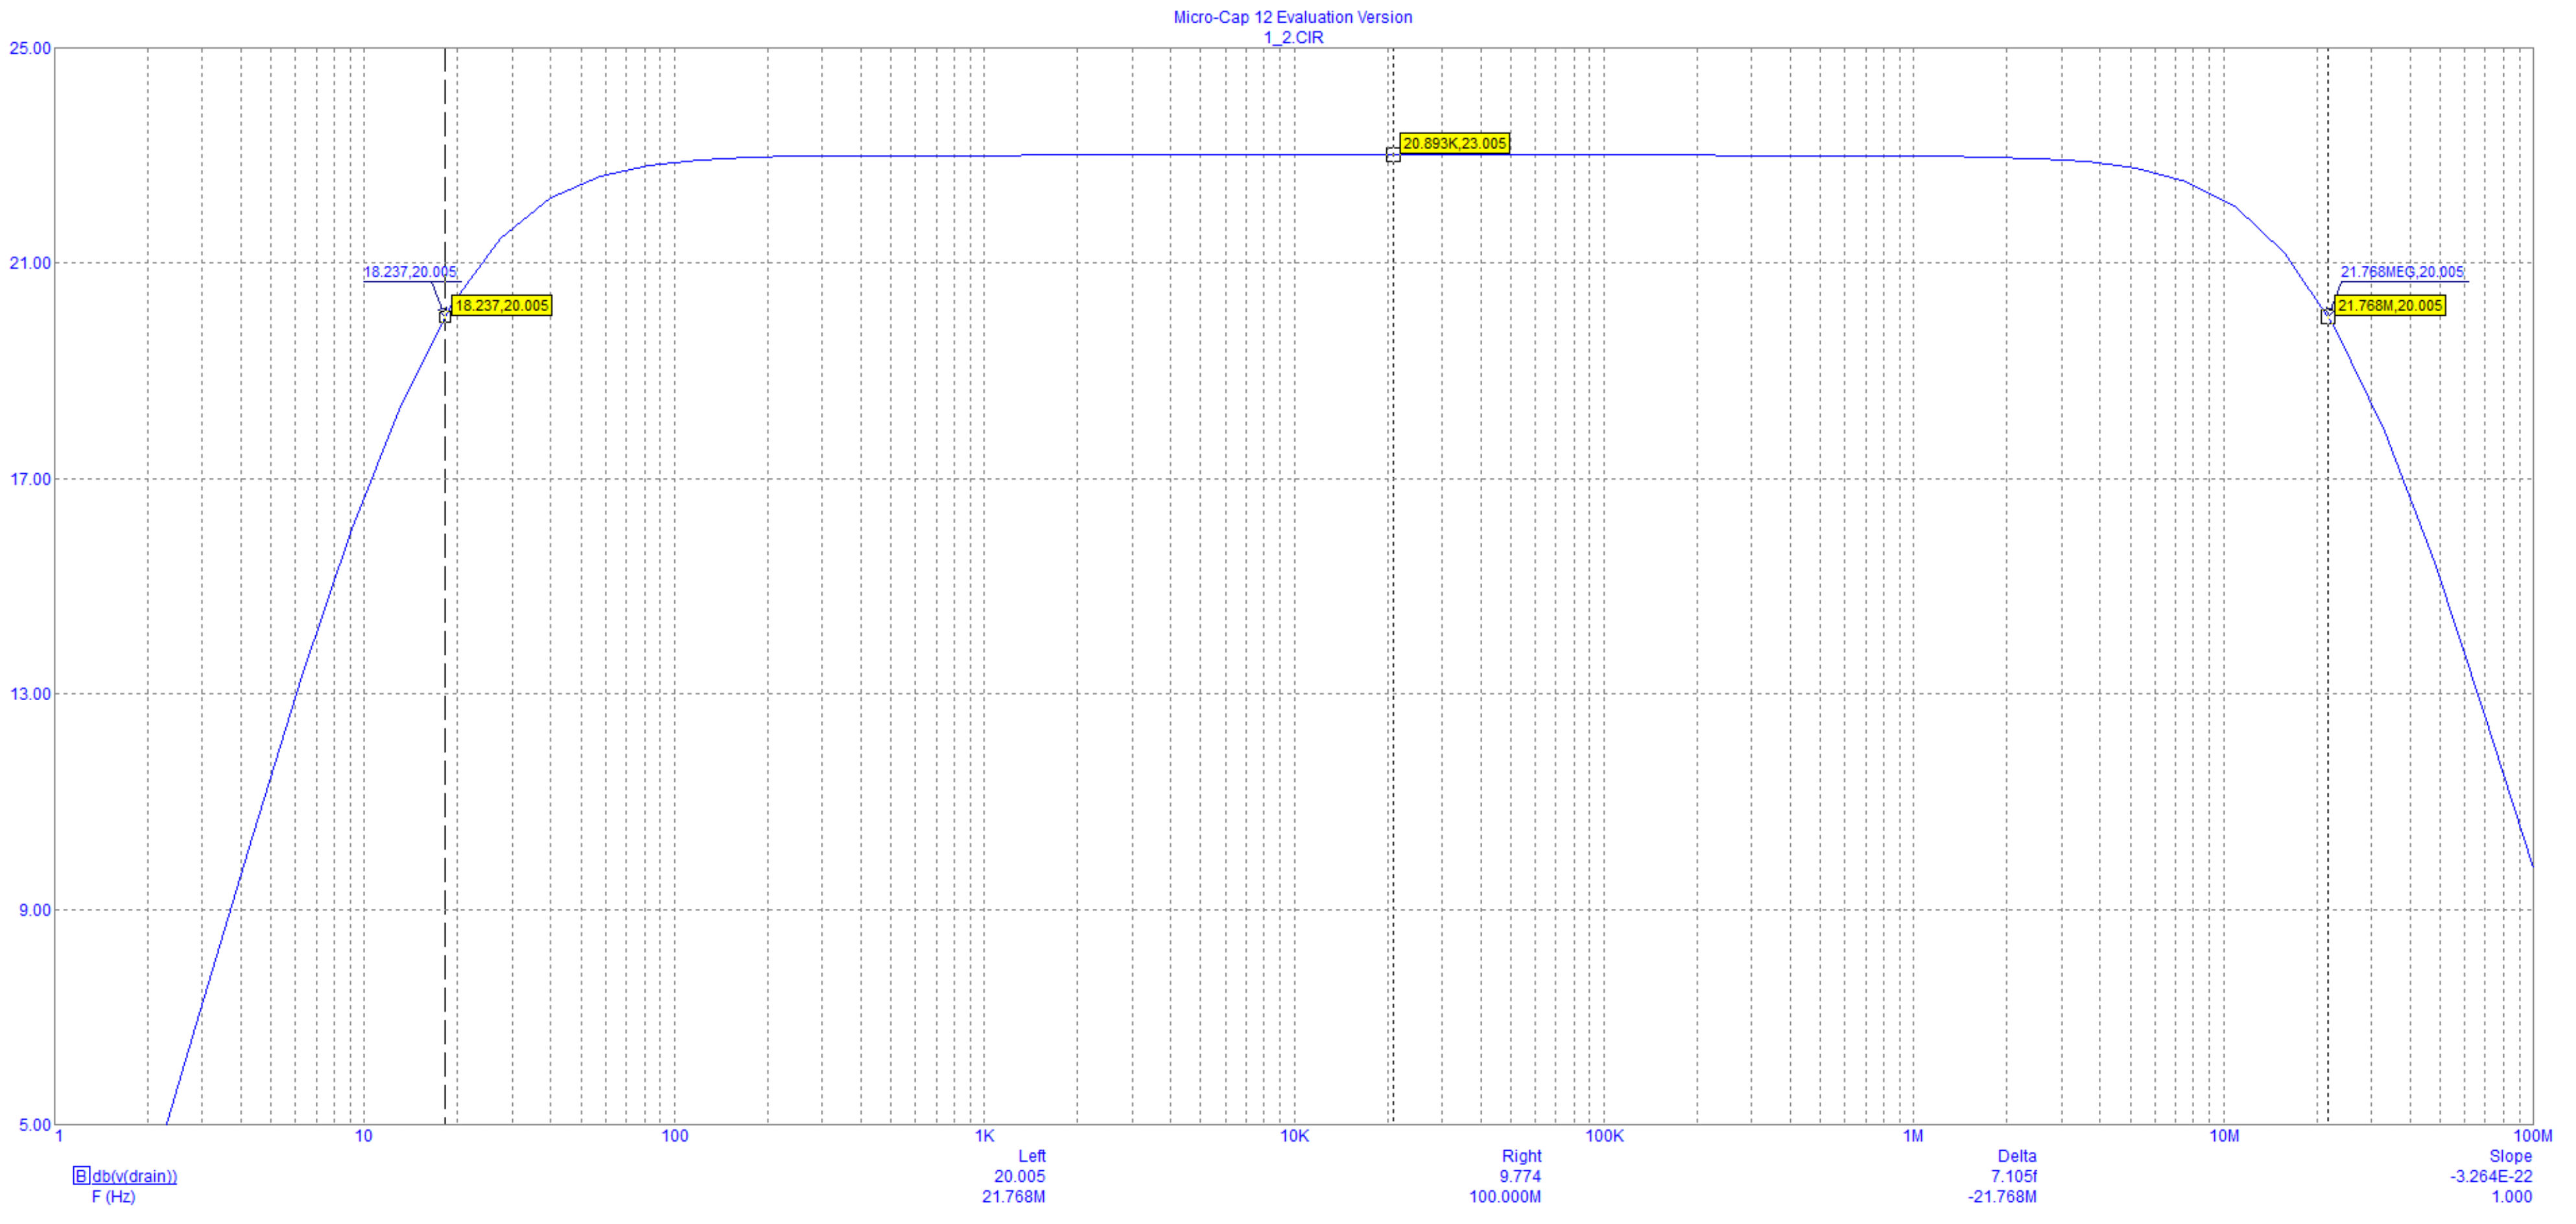
\includegraphics[width=\textwidth]{PC/UNI/UNI_sirka_pasma_2.png}
      \caption{\label{sirka_pasma} Šířka pásma při \(C_v = 5\-[\mu F]\)}
    \end{figure}
    \begin{figure}[H]
      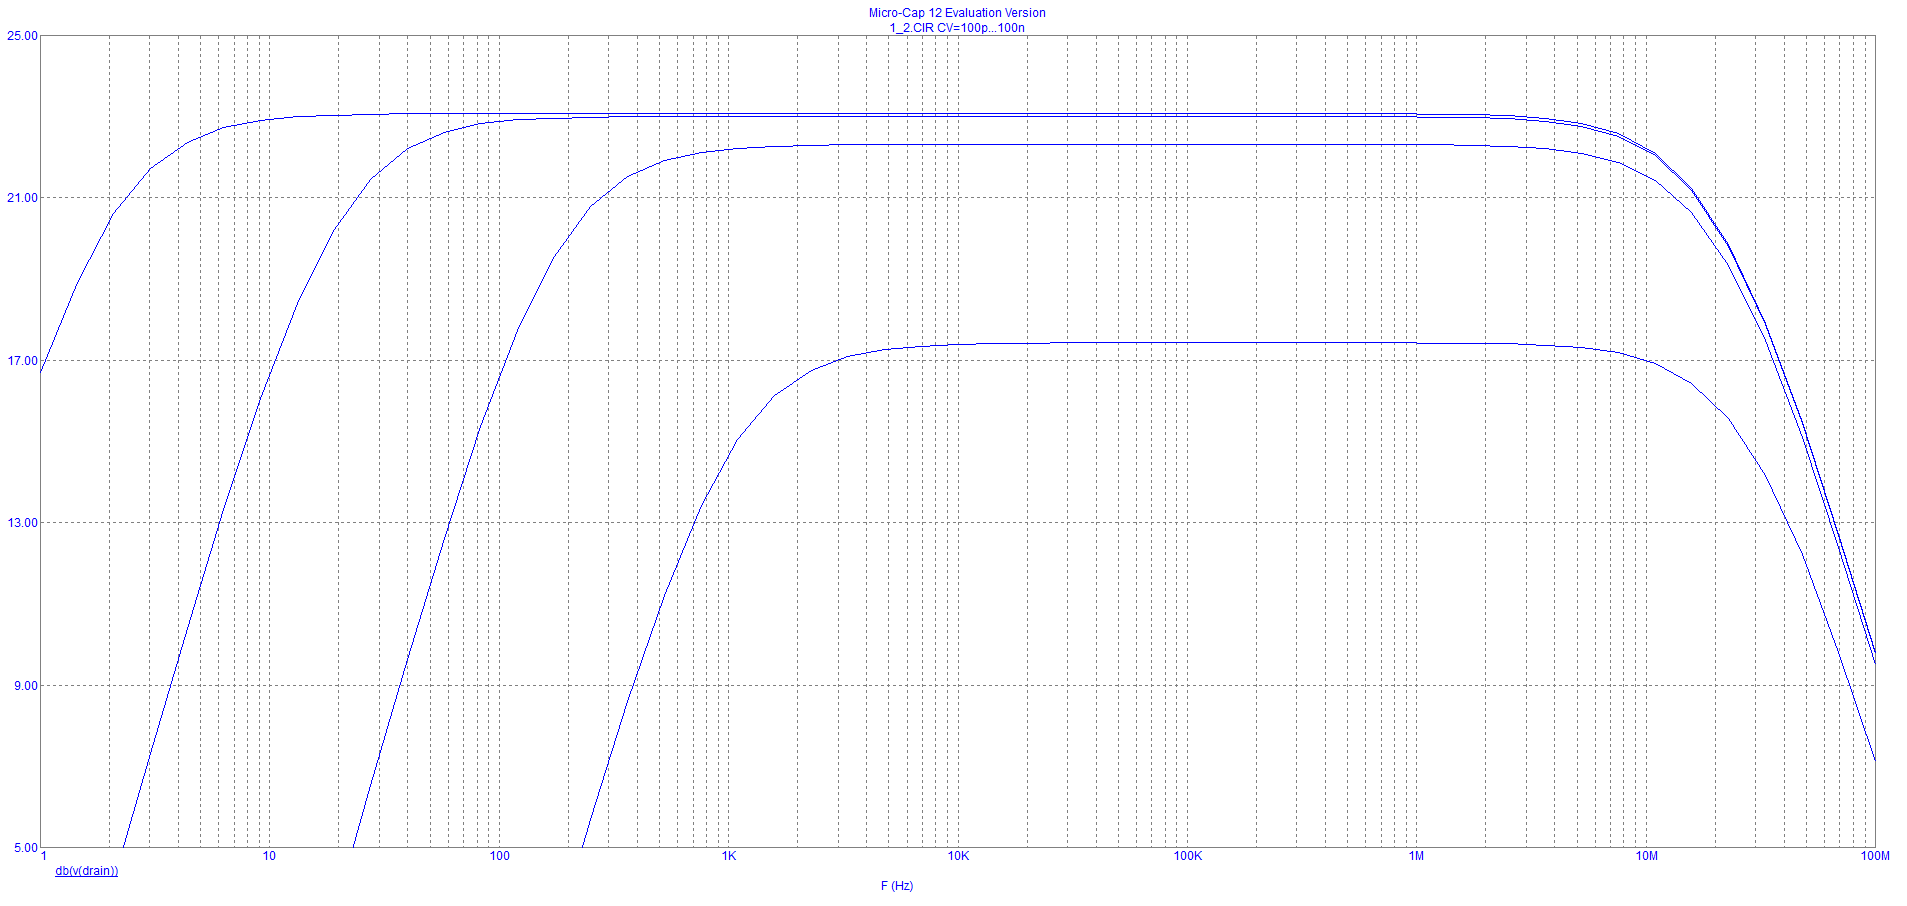
\includegraphics[width=\textwidth]{PC/UNI/UNI_sirky_pasma.png}
      \caption{\label{Pohyb_sirky_pasma} Šířka pásma při změně \(C_v = 0.1;1;10\-[\mu F]\)}
    \end{figure}
  \end{minipage}

  \begin{minipage}[t]{1\textwidth}
    \vspace{5mm}
    Je vidět, že zmenšení kapacitoru znamená omezení šířky pásma v dolní části, nikoliv v horní.
    Na rozdíl od bipolárního tranzistoru, kde se zmenšuje šířka pásma, ale maximální zesílení zůstává stejné.
    V tomto zapojení zvýšení kapacity znamená zároveň zvýšení maximálního zesílení.
    To proto, že mezi elektrodami \(G\) a \(S\) u unipolárního tranzistoru je parazitní kapacita, která společně s \(C_v\) tvoří napěťoví dělič.
    Odpor mezi elektrodou \(G\) a zemí, který je u \(f\) blížící se \(0\) roven pouze \(R_{G2}\) se zvyšující frekvencí zmenšuje kvůli parazitní kapacitě \(C_{GS}\).
  \end{minipage}
\end{figure}

\newpage
\section{Laboratorní cvičení}
% \subsections{zadání}
% Nejprve sestavte obvod bez vazebního kondenzátoru a zdroje signálu. Změnou odporu Rb
% nastavte ss napětí na kolektoru tranzistoru 6 V. Změřte všechna uzlová napětí a z nich dopočtěte
% větvové proudy. Porovnejte s výsledky z NC a PC.
% Doplňte obvod o Cv a generátor signálu. Proveďte „oživení“ zesilovače pomocí osciloskopu.
% Zesilovač nesmíte přebudit výstupní napětí nesmí vykazovat zkreslení. Měřte při kmitočtu
% 1 kHz. Zakreslete časové průběhy vstupního napětí, napětí na bázi a na kolektoru, včetně ss
% posunutí. Změřte amplitudy a vypočtěte z nich střídavá zesílení.

\begin{figure}[H]
	\begin{minipage}[t]{0.6\textwidth}
    Měřili jsme s tranzistorem BC55, u kterého jsme na začátku naměřili \(\beta = 422\)
    Nejprve jsme sestavili obvod a pomocí potenciometru jsme nastavili pracovní bod dle \tab{tab_pracovni_bod}.
    % \vspace{-5mm}
    \begin{table}[H]
      % \centering
      \begin{tabular}{|c|c|c|c|c||c|c|} 
        \hline
         \(U_{cc}\-[V]\) & \(U_{C}\-[V]\)  & \(R_b\-[M\Omega]\) &	\(R_c\-[K\Omega]\) & \(U_{b}\-[V]\) & \(I_{C}\-[mA]\) & \(I_{b}\-[\mu A]\)  \\ \hline
         12              & 6.1             & 2.5                & 2.2                & 0.61           & 2.68            & 6.36                \\ \hline
      \end{tabular}
      \caption{\label{tab_pracovni_bod} Nastavení obvodu}
    \end{table}
   	\(\bullet\) kanál 1 ... \(U_{in}\)  \qquad 	\(\bullet\) kanál 2 ... \(U_{out}\)
  \end{minipage}
  \hfill
	\begin{minipage}[t]{0.4\textwidth}
    \begin{figure}[H]
      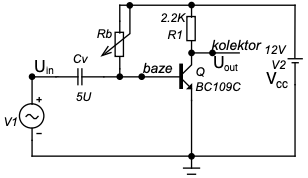
\includegraphics[width=\textwidth]{obvod-z-laborky.png}
      \caption{\label{obvod_z_laborky}}
    \end{figure}
  \end{minipage}
\end{figure}


\begin{figure}[H]
	\begin{minipage}[t]{0.6\textwidth}
    \vspace{-20mm}
    \begin{figure}[H]
      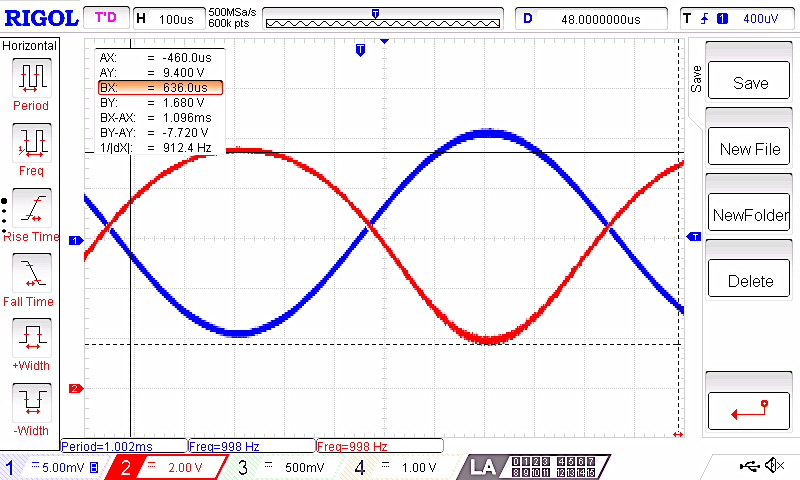
\includegraphics[width=\textwidth]{LAB/NewFile2.png}
      \caption{\label{obvod_z_laborky}}
    \end{figure}
  \end{minipage}
  \hfill
	\begin{minipage}[t]{0.35\textwidth}
    Dále jsme na vstup přivedly signál o napětí \(U_{in} = 1\-[V]\) a frekvenci \(f = 1\-[kHz]\). 
    Díky hodnotě vstupního napětí \(U_{in} = 1\-[V]\) rovnou vidíme zesílení tohoto zapojení \(K_u = 7.72\-[-]\).
  \end{minipage}
\end{figure}

\begin{figure}[H]
	\begin{minipage}[t]{0.6\textwidth}
    \vspace{-10mm}
    \begin{figure}[H]
      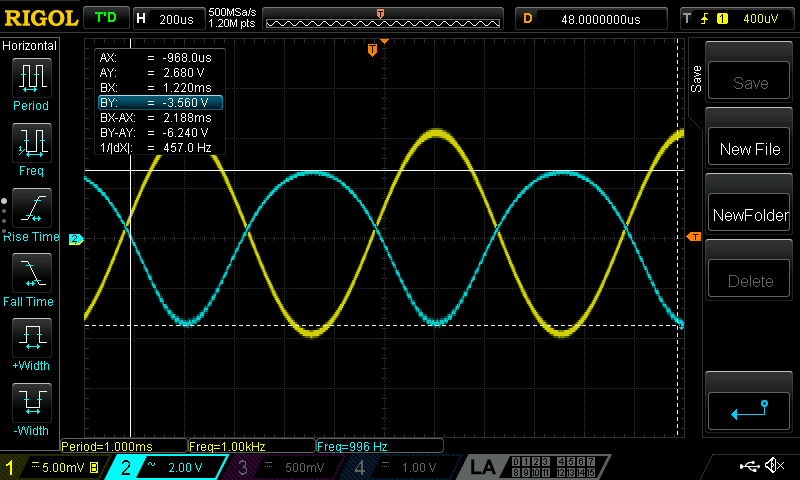
\includegraphics[width=\textwidth]{LAB/NewFile4.png}
      \caption{\label{obvod_z_laborky}}
    \end{figure}
  \end{minipage}
  \hfill
	\begin{minipage}[t]{0.35\textwidth}
    % Dále jsme přenastavili pracovní bod dle tabulky:
    \begin{table}[H]
      % \centering
      \vspace{8mm}
      \hspace{-5mm}
      \small
      \begin{tabular}{|c|c|c|c|c|} 
        \hline
        \(U_{cc}\-[V]\) & \(U_{C}\-[V]\)  & \(R_b\-[M\Omega]\) & \(R_c\-[K\Omega]\) & \(U_{b}\-[V]\)  \\ \hline
        12              & 7.6             & 3.44               & 2.2                & 0.61            \\ \hline
        \hline
        \(I_{C}\-[mA]\) & \(I_{b}\-[\mu A]\) & - & - & - \\\hline
        2.00            & 4.74               & - & - & - \\\hline
      \end{tabular}
      \normalsize
      \caption{\label{tab_pracovni_bod_rozladeni1} Přenastavení obvodu 1}
    \end{table}
  \end{minipage}
\end{figure}

\vspace{-1mm}
\begin{figure}[H]
	\begin{minipage}[t]{0.6\textwidth}
    \vspace{-13mm}
    \begin{figure}[H]
      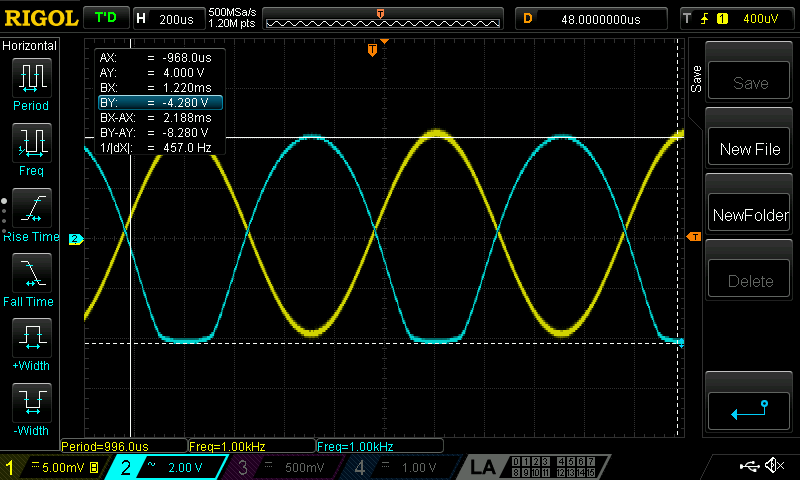
\includegraphics[width=\textwidth]{LAB/NewFile6.png}
      \caption{\label{obvod_z_laborky}}
    \end{figure}
  \end{minipage}
  \hfill
	\begin{minipage}[t]{0.35\textwidth}
    % Dále jsme přenastavili pracovní bod dle tabulky:
    \begin{table}[H]
      % \centering
      \vspace{8mm}
      \hspace{-5mm}
      \small
      \begin{tabular}{|c|c|c|c|c|} 
        \hline
        \(U_{cc}\-[V]\) & \(U_{C}\-[V]\)  & \(R_b\-[M\Omega]\) & \(R_c\-[K\Omega]\) & \(U_{b}\-[V]\)  \\ \hline
        12              & 4.5             & 1.90               & 2.2                & 0.61            \\ \hline
        \hline
        \(I_{C}\-[mA]\) & \(I_{b}\-[\mu A]\) & - & - & - \\\hline
        3.41            & 8.08               & - & - & - \\\hline
      \end{tabular}
      \normalsize
      \caption{\label{tab_pracovni_bod_rozladeni1} Přenastavení obvodu 2}
    \end{table}
  \end{minipage}
\end{figure}


\begin{figure}[H]
  \begin{minipage}[t]{\textwidth}
    \vspace{-7mm}
    \begin{tikzpicture}
      \begin{semilogxaxis}[
            width=1\textwidth, 
            height=100mm,
            title={Šířka pásma při změně \(C_v\)},
            xlabel={\(f\-[Hz]\)},
            ylabel={\(K_u~[-]\)},
            xmin=1, xmax=5000000,
            ymin=-14, ymax=20,
            legend pos=south east,
        ]
        \addplot[
          color=red,
          mark=x,
          ]
          coordinates {
            (1       , -21.94)
            (2       , -16.48)
            (5       , -15.92)
            (10      , -14.89)
            (20      , -13.56)
            (50      , -11.70)
            (100     ,  -6.94)
            (200     ,  -1.94)
            (500     ,   5.11)
            (1000    ,   9.94)
            (2000    ,  13.84) %
            (5000    ,  16.44)
            (10000   ,  16.90)
            (20000   ,  17.00)
            (50000   ,  16.28)
            (100000  ,  15.50)
            (200000  ,  14.52)
            (500000  ,  11.95) %
            (1000000 ,   7.75)
            (2000000 ,   2.41)
            (5000000 ,  -5.19)
          };
          \addlegendentry{\scriptsize \(C_v = 10\-[nF]\)}
        \addplot[
          color=orange,
          mark=x,
          ]
          coordinates {
            (1       , -13.98)
            (2       , -12.04)
            (5       , -10.75)
            (10      ,  -7.54)
            (20      ,  -2.16)
            (50      ,   4.71)
            (100     ,   9.83)
            (200     ,  14.12) %
            (500     ,  16.95)
            (1000    ,  17.48)
            (2000    ,  17.66)
            (5000    ,  17.84)
            (10000   ,  17.93)
          };
          \addlegendentry{\scriptsize \(C_v = 100\-[nF]\)}
        \addplot[
          color=yellow,
          mark=x,
          ]
          coordinates {
            (1       , -7.79)
            (2       , -2.76)
            (5       ,  4.65)
            (10      ,  9.99)
            (20      , 14.01) %
            (50      , 17.00)
            (100     , 17.57)
            (200     , 17.75)
            (500     , 17.93)
          };
          \addlegendentry{\scriptsize \(C_v = 1\-[\mu F]\)}
        \addplot[
          color=blue,
          mark=x,
          ]
          coordinates {
            (1       ,  6.69)
            (2       , 12.38) %
            (5       , 16.44)
            (10      , 17.34)
            (20      , 17.57)
            (50      , 17.75)
            (100     , 17.84)
            (200     , 17.84)
            (500     , 17.93)
          };
          \addlegendentry{\scriptsize \(C_v = 10\-[\mu F]\)}
        \addplot[
          color=green,
          mark=x,
          ]
          coordinates {
            (1       ,  1.87)
            (2       ,  8.43)
            (5       , 14.45) %
            (10      , 16.60)
            (20      , 17.29)
            (50      , 17.66)
            (100     , 17.80)
            (200     , 17.80)
            (500     , 17.93)
            (1000    , 17.93)
            (2000    , 17.93)
            (5000    , 17.93)
            (10000   , 17.93)
            (20000   , 17.62)
            (50000   , 16.90)
            (100000  , 16.12)
            (200000  , 15.09)
            (500000  , 12.21) %
            (1000000 ,  8.30)
            (2000000 ,  3.41)
            (5000000 , -6.02)
          };
          \addlegendentry{\scriptsize \(C_v = 4.7\-[\mu F]\)}
          \addplot[
            color=black,
            mark=o,
          ]
          coordinates {
            (5       , 14.45) %
            (5       , -100) %
            (500000  , -100) %
            (500000  , 12.21) %
          };
          \addplot[
            color=black,
            mark=o,
          ]
          coordinates {
            (2       , 12.38) %
            (2       ,  -100) %
          };
          \addplot[
            color=black,
            mark=o,
          ]
          coordinates {
            (20      , -100) % 
            (20      , 14.01) %
          };
          \addplot[
            color=black,
            mark=o,
          ]
          coordinates {
            (200     , -100) %
            (200     , 14.12) %
          };
          \addplot[
            color=black,
            mark=o,
          ]
          coordinates {
            (2000    ,  13.84) %
            (2000    , -100  ) %
            (500000  , -100  ) %
            (500000  ,  11.95) %
          };
      \end{semilogxaxis}
    \end{tikzpicture}
  \end{minipage}
  Zvýrazněna jsou ta měření která jsou jak první mimo šířku pásma.
  Měření potvrzuje teorii, že velikost oddělovacího kapacitoru \(C_v\) ovlivňuje šířku pásma jen ve spodní části.
  Příliš velká hodnota \(C_v\) však šířku pásma omezí natolik, že zesílení nestihne stoupnout na maximum a už se začne oslabovat, což vidíme u průběhu s kapacitorem \(C_v = 10\-[nF]\). 
\end{figure}



\begin{figure}[H]
  \begin{minipage}[t]{\textwidth}
    \section{Závěr}
    Ze všech těchto úkolu plyne, že nastavení pracovního bodu musí odpovídat potřebám konkrétního zapojení, jinak dojde ke zkreslení zesilovaného signálu.
    To vetšinou znamená mít napětí mezi kolektorem a zemí \(U_C = \frac{1}{2}U_{cc}\).
    Signál, který podobné zapojení zesiluje, také nesmí mít příliš velkou amplitudu, jinak dojde k saturaci tranzistoru a tím pádem ke zkreslení signálu.

    Kondenzátor \(C_V\) na vstupu určuje spodní hranici šířky pásma, dá se tedy použít jako horní propusť a nebo naopak může být problém u nízkofrekvenčních aplikací.

  \end{minipage}
\end{figure}

\end{document}
